\documentclass[a4paper, oneside]{article}

\usepackage[T1]{fontenc}
\usepackage[utf8]{inputenc}
\usepackage[english]{babel}
\usepackage{frontespizio}
\usepackage{graphicx}
\usepackage{listings}
\usepackage{scrextend}
\usepackage[margin=1.2in]{geometry}
\usepackage[font=small,labelfont=bf]{caption}

\begin{document}
\selectlanguage{english}
\baselineskip 13pt

% ---- FRONTESPIZIO ----- 
\begin{frontespizio} 
 \Preambolo{\renewcommand{\frontpretitlefont}{\fontsize{15}{12}\scshape}}
\Istituzione {University of Pisa}
\Divisione {Scuola di Ingegneria}
\Corso [Laurea]{Artificial Intelligence and Data Engineering}
\Annoaccademico {2019--2020}
\Titolo {Task2 documentation}
\Filigrana [height=4cm,before=0.28,after=1]{./images/stemma_unipi.png}
\Rientro {1cm}
\Candidato {Alice Nannini}
\Candidato {Giacomo Mantovani}
\Candidato {Marco Parola}
\Candidato {Stefano Poleggi}
\Relatore {Prof. Pietro Ducange}
 \Punteggiatura {}
\end{frontespizio}

\clearpage

% ----- INDICE -----
	\tableofcontents\thispagestyle{empty}
	\clearpage


\section{Introduction}\pagenumbering{arabic}
The \textbf{Cine-Valutami} application offers a search and consultation service in the field of cinema. When the application starts, the system requires authentication to use the service.
The logged-in user can perform a search by entering the first characters of a film title in the search bar, obtaining a list of 10 films in the database. After that you can select one of the proposed titles or carry out a more in-depth search, adding characters.
At the time of selection, the system allows you to view more information in the section on the right, including cover, title, director and rating.
The user can leave a mark from 1 to 5 for the selected film.
There is also a module for the system administrator, who will be redirected to an activity different from that of the user, in which he can view some statistics linked to the films and to the searches carried out by the users of the application, in particular: ranking of 10 most voted films, ranking of the 10 most sought after films.
Besides, the system administrator can add new films to the application database or delete those already present, by searching by title.
\begin{minipage}{\linewidth}
\begin{center}
\vspace{8mm}
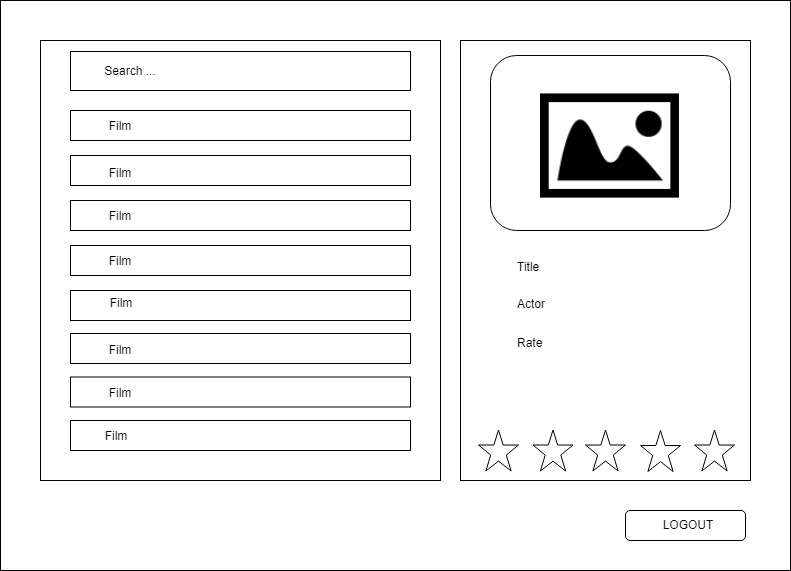
\includegraphics[width=\textwidth]{./images/diagrams/UserMockup} 
\vspace{3mm}
\captionof{figure}{Mockup}
\label{fig:mockup}
\end{center}
\end{minipage}

\clearpage

\section{Analysis and workflow}

% ----- REQUIREMENTS -----
\subsection{Requirements}


\subsubsection{Functional requirement}
The system has to allow the user to carry out basic functions such as:
\begin{itemize}
\item To sign up into the system.
\item To login into the system.
\item To search for a film.
\item To vote a film.
\end{itemize}
\vspace{2mm}
The system has to allow the administrator to carry out basic functions such as:
\begin{itemize}
\item To login into the system.
\item To add a film.
\item To update a film.
\item To delete a film.
\item To view a list of top rated films.
\item To view the a list of the most searched films.
\end{itemize}
\vspace{2mm}

\subsubsection{Non-functional requirements}
\begin{itemize}
\item Usability, ease of use and intuitiveness of the application by the user.
\item Avaliablility, with the service guaranteed h24.
\item The system should support simultaneous users.
\item The system should provide access to the database with a few seconds of latency.
\end{itemize}

\clearpage

% ----- USE CASES -----
\subsection{Use case}

\textbf{Actors}
\begin{itemize}
\item{User : this actor represents a user of the system}
\item{Admin : this actor represents the administrator of the system}
\end{itemize}

\subsubsection{Use Cases Description}
\begin{table}[h]
\centering
\begin{tabular}{p{0.2\textwidth}p{0.1\textwidth}lp{0.5\textwidth}}
\hline
\textbf{Event} & \textbf{UseCase} & \textbf{Actor(s)} & \textbf{Description}\\ \hline
Log in, Log out & Login,  Logout & Admin, User & The user logs in/out the application.\\ \hline
Display all the Films & Browse, Find, Display Films & User, Admin & The user chooses that he wants to view the list of Films. The system browses the data on the db and returns them on the interface.\\ \hline
View Statistics & View Statistic, View Top Rated Films, View Most Searched Films & Admin & The Admin clicks on button to view the statistics. The system browses on the db the informations used in the calculation and display the result.\\ \hline
Add a film & Add Film & Admin & The admin submits the Film informations. The system updates the db and the interface.\\ \hline
Update a film & Update Film & Admin & The admin selects the film and commits the new informations. The system updates the db and the interface.\\ \hline
Delete a film & Delete Film & Admin & The admin selects the film and submits the delete. The system updates the db and the interface.\\ \hline
View the film informations & Select Film, Display Info Film & User, Admin & The user selects the film. The system shows the film informations on the interface.\\ \hline
Vote a film & Vote Film & User, Admin & The user submits the vote on a selected film. The system updates the db and the interface.\\ \hline
\end{tabular}
\end{table}

\begin{minipage}{\linewidth}
\begin{center}
\vspace{8mm}
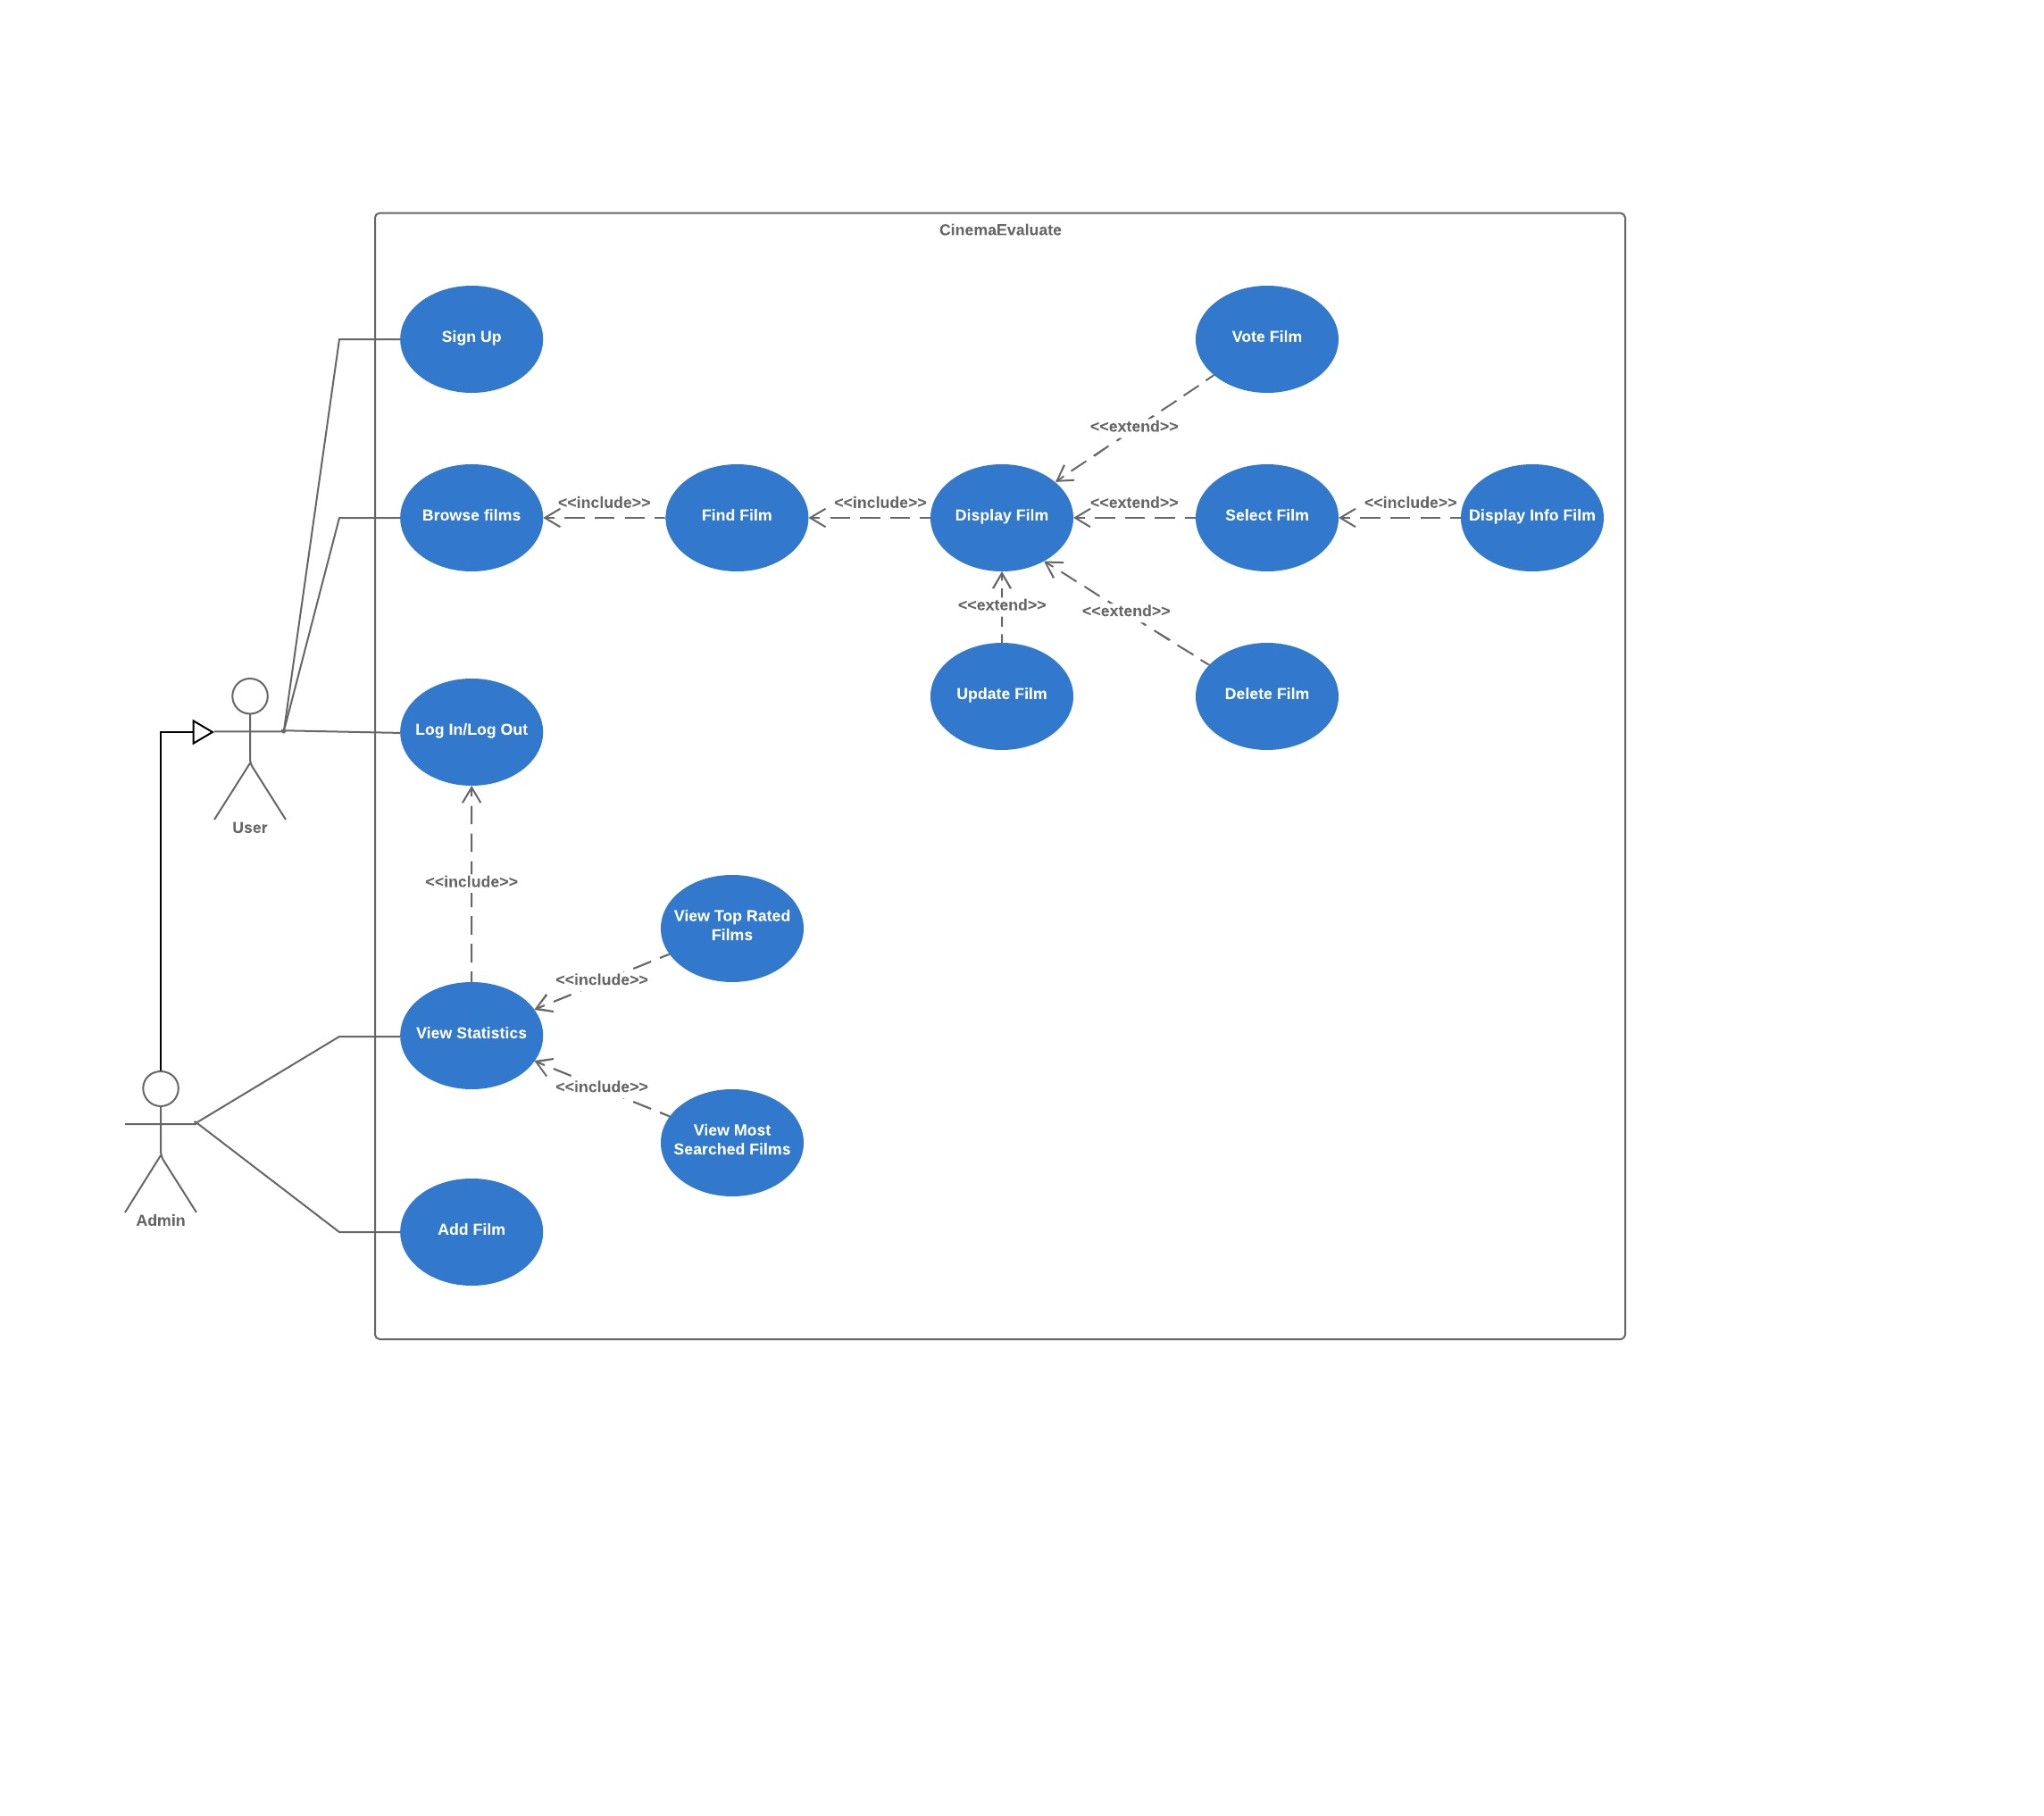
\includegraphics[ width=0.8\textheight]{./images/diagrams/CinemaEvaluate} 
\captionof{figure}{Use cases diagram}
\vspace{3mm}
\end{center}
\end{minipage}


\clearpage


\subsection{Class diagram}
This diagram represent the main entities of the application and the relations between them.
\begin{minipage}{\linewidth}
\begin{center}
\vspace{4mm}
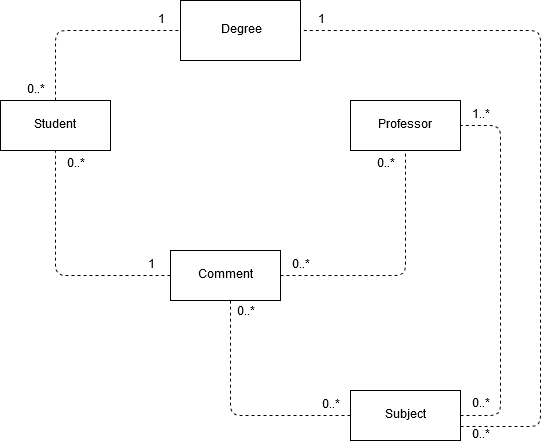
\includegraphics[width = 0.7\textwidth]{./images/diagrams/AnalysisUML.png} 
\vspace{2mm}
\captionof{figure}{UML analysis diagram}
\label{fig:useCases}
\end{center}
\end{minipage}



\clearpage
% ----- DESIGN -----
\section{Design}

\subsection{Software architecture}
The application is designed over 3 different layers, see figure \ref{fig:architecture_diagram}:
\begin{itemize}
\item Front-end
\item Middleware
\item Back-end
\end{itemize}
\vspace{5mm}
\begin{minipage}{\linewidth}
\begin{center}
\vspace{1mm}
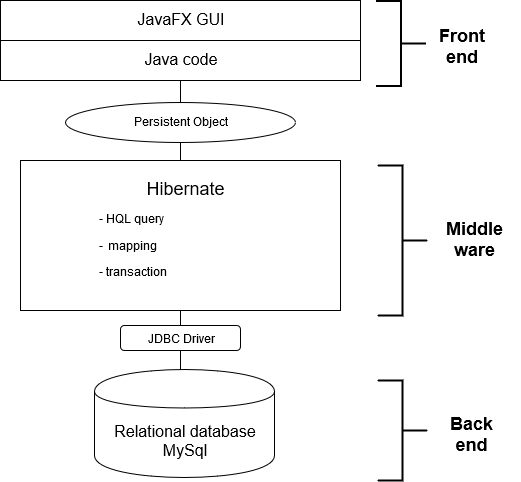
\includegraphics[height = 100mm]{./images/diagrams/architecture_diagram.png} 
\vspace{6mm}
\captionof{figure}{Software architecture diagram\\}
\label{fig:architecture_diagram}
\end{center}
\end{minipage}
\vspace{5mm}

\iffalse

\clearpage
\subsection{Database design}
The application is developped over a relational-database, using the MySql platform. The figure \ref{fig:diagramma_er} shows the ER-diagram of the database.\\

\begin{minipage}{\linewidth}
\begin{center}
\vspace{1mm}
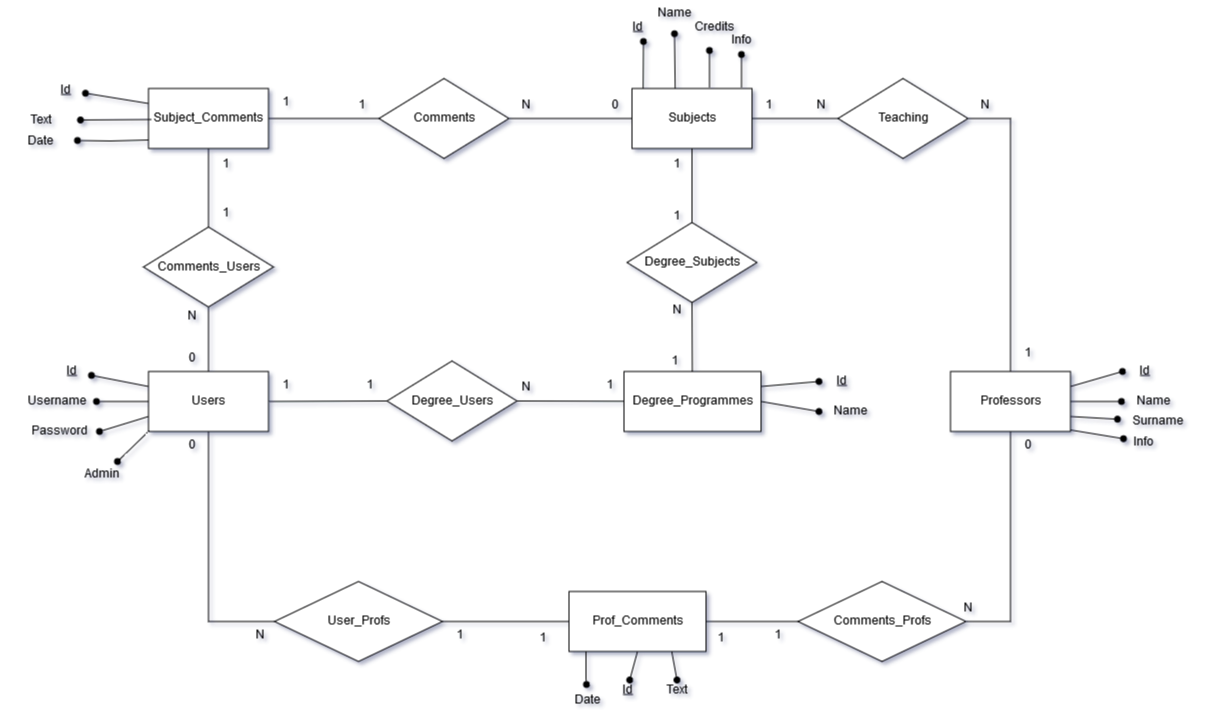
\includegraphics[width=155mm]{./images/diagrams/er_diagram.png} 
\vspace{2mm}
\captionof{figure}{ER diagram\\}
\label{fig:diagramma_er}
\end{center}
\end{minipage}

\vspace{19mm}



\clearpage
% ----- IMPLEMENTATION -----



\section{Implementation}
\subsection{Used technologies}
The application is developed in java programming language, version 11.0.4, and in JavaFX system to create the GUI, version 11, so it should run on each platform in which JVM is installed, but the application is tested and guardantee on Ubuntu 16 and Window OS. Moreover Maven is used  to build and mantain the project, version 3.8.0. \\
The middleware layer is built thanks to Hibernate, version 5.4.4.0.\\
The jdbc driver manage the comunication between middleware layer and backend layer, version 8.0.17.\\ 
For the backend layer it is used Apache as web-server, version 2.4 (including Php, MySql).\\
So this application is tested using these technologies, considering these particular versions: for other versions the correct execution isn't guaranteed .
\subsection{Snippets of code}
This phase describes the most interesting parts about the creation and interaction with the database.\\
The following classes are mapped in the table of the database: 

\begin{itemize}	
\item Degree
\item Student
\item Professor
\item Subject
\item ProfessorComment
\item ProfessotSubject
\end{itemize}


\begin{itemize}	
\item Degree
\item Student
\item Professor
\item Subject
\item ProfessorComment
\item ProfessotSubject
\end{itemize}
These classes are declared using the Hibernate annotations syntax.\\

\subsubsection{Declaretion of class Subject}
The following java-code shows a declaration of the class Subject.
\vspace{2mm}
% ----- android wearable module -----
\begin{lstlisting}[language=Java,  basicstyle=\footnotesize]
@Entity(name = "Subjects")
@Table(name = "subjects")
public class Subject {

	@Column(name = "id")
	@Id
	@GeneratedValue(strategy = GenerationType.IDENTITY)
	private int id;
	private String name;
	private int credits;
	@Column(name = "info", columnDefinition="TEXT")
	private String info;

	// relation with degree
	@ManyToOne(fetch = FetchType.LAZY)
	@JoinColumn(name = "degreeId")
	private Degree deg;

	// relation with Subject comments.
	@OneToMany(mappedBy = "subj", cascade = CascadeType.ALL, orphanRemoval = true)
	private List<SubjectComment> subjectComments = new ArrayList<SubjectComment>();

	// relation with Professors.
	@ManyToMany
	@JoinTable(name = "teaching", joinColumns = @JoinColumn(name = "subjectId"),
		 inverseJoinColumns = @JoinColumn(name = "profId"))
	private Set<Professor> professor = new HashSet<Professor>();
\end{lstlisting}
\vspace{5mm}


\subsubsection{Declaretion of class Person}
The following java-code shows a declaration of the class Person. The @MappedSuperclass annotation is used to map the superclass.
\vspace{2mm}
% ----- android wearable module -----
\begin{lstlisting}[language=Java,  basicstyle=\footnotesize]
@MappedSuperclass
public abstract class Person {

	@Column(name = "id")
	@Id
	@GeneratedValue(strategy = GenerationType.IDENTITY)
	private int id;
   ...
}
\end{lstlisting}
\vspace{5mm}


\subsubsection{Declaretion of class Professor}
The following java-code shows a declaration of the class Professor.
\vspace{2mm}
% ----- android wearable module -----
\begin{lstlisting}[language=Java,  basicstyle=\footnotesize]
@Entity(name = "Professors")
@Table(name = "professors")
public class Professor extends Person {

	@Column(name = "info", columnDefinition="TEXT")
	private String info;
	private String name;
	private String surname;

	// relation with profComments.
	@OneToMany(mappedBy = "prof", cascade = CascadeType.ALL, orphanRemoval = true, 
								fetch = FetchType.LAZY)
	private List<ProfessorComment> professorComments = new ArrayList<ProfessorComment>();

	// relation with Subjects.
	@ManyToMany(mappedBy = "professor", cascade = CascadeType.ALL)
	private Set<Subject> subject = new HashSet<Subject>();
   ...
}
\end{lstlisting}
\vspace{5mm}


\subsubsection{Declaretion of class Student}
The following java-code shows a declaration of the class Student.
\vspace{2mm}
% ----- android wearable module -----
\begin{lstlisting}[language=Java,  basicstyle=\footnotesize]
@Entity(name = "Users")
@Table(name = "users")
public class Student extends Person {

	private final boolean admin;
	@Column(name = "username", unique = true)
	private String username;
	private String password;

	// relation with Degree.
	@ManyToOne(fetch = FetchType.LAZY)
	@JoinColumn(name = "degreeId")
	private Degree deg;

	// relation with SubjectComments.
	@OneToMany(mappedBy = "stud", cascade = CascadeType.ALL, orphanRemoval = true)
	private List<SubjectComment> subjectComments = new ArrayList<SubjectComment>();

	// relation with ProfessorComments.
	@OneToMany(mappedBy = "stud", cascade = CascadeType.ALL, orphanRemoval = true)
	private List<ProfessorComment> professorComments = new ArrayList<ProfessorComment>();
   ...
}
\end{lstlisting}
\vspace{5mm}


\subsubsection{Declaretion of class Comment}
The following java-code shows a declaration of the class Comment. The @MappedSuperclass annotation is used to map the superclass.
\vspace{2mm}
% ----- android wearable module -----
\begin{lstlisting}[language=Java,  basicstyle=\footnotesize]
@MappedSuperclass
public abstract class Comment {

	@Column(name = "id")
	@Id
	@GeneratedValue(strategy = GenerationType.IDENTITY)
	private int id;
	private String text;
	private String date;
        
        private static String format = "yyyy-MM-dd HH:mm:ss";
   ...
}
\end{lstlisting}
\vspace{5mm}


\subsubsection{Declaretion of class SubjectComment}
The following java-code shows a declaration of the class SubjectComment.
\vspace{2mm}
% ----- android wearable module -----
\begin{lstlisting}[language=Java,  basicstyle=\footnotesize]
@Entity(name = "SubjectComments")
@Table(name = "subject_comments")
public class SubjectComment extends Comment {

	@ManyToOne(fetch = FetchType.LAZY)
	@JoinColumn(name = "userId")
	private Student stud;

	@ManyToOne(fetch = FetchType.LAZY)
	@JoinColumn(name = "subjectId")
	private Subject subj;
   ...
}
\end{lstlisting}
\vspace{5mm}


\subsubsection{Declaretion of class ProfessorComment}
The following java-code shows a declaration of the class ProfessorComment.
\vspace{2mm}
% ----- android wearable module -----
\begin{lstlisting}[language=Java,  basicstyle=\footnotesize]
@Entity(name = "ProfComments")
@Table(name = "prof_comments")
public class ProfessorComment extends Comment {

	@ManyToOne(fetch = FetchType.LAZY)
	@JoinColumn(name = "profId")
	private Professor prof;

	@ManyToOne(fetch = FetchType.LAZY)
	@JoinColumn(name = "userId")
	private Student stud;
   ...
}
\end{lstlisting}
\vspace{5mm}


\subsubsection{Declaretion of class Degree}
The following java-code shows a declaration of the class Degree.
\vspace{2mm}
% ----- android wearable module -----
\begin{lstlisting}[language=Java,  basicstyle=\footnotesize]
@Entity(name = "Degree")
@Table(name = "degree_programmes")
public class Degree {

	@Column(name = "id")
	@Id
	@GeneratedValue(strategy = GenerationType.IDENTITY)
	private int id;

	@Column(name = "name", unique = true)
	private String name;

	// relation with students.
	@OneToMany(mappedBy = "deg", cascade = CascadeType.ALL, orphanRemoval = true)
	private List<Student> student = new ArrayList<Student>();

	// relation with subjects.
	@OneToMany(mappedBy = "deg", cascade = CascadeType.ALL, orphanRemoval = true)
	private List<Subject> subject = new ArrayList<Subject>();
   ...
}
\end{lstlisting}
\vspace{5mm}

\begin{minipage}{\linewidth}
\begin{center}
\vspace{1mm}
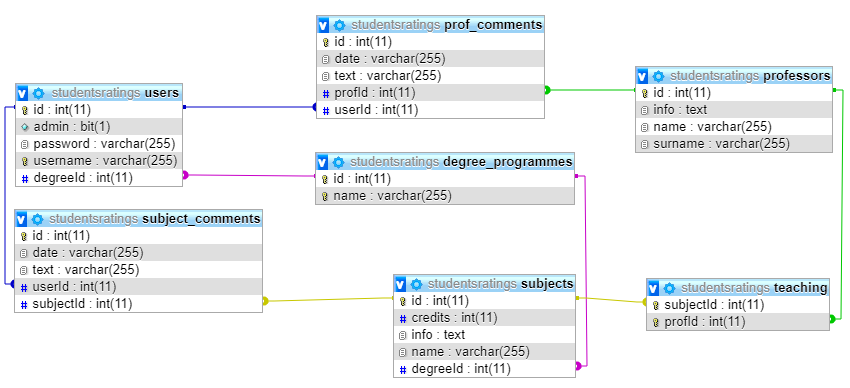
\includegraphics[width=155mm]{./images/diagrams/er_diagram2.png} 
\captionof{figure}{ER diagram\\}
\label{fig:diagramma_er2}
\end{center}
\end{minipage}
\vspace{5mm}\\
 Another foundamental class is ManagerEM, that manages the db-connection and the related operations.
 The implementation of a set of CRUD operations, regarding the class Subject, is desribed as follows.

\subsection{Create}
Creating a new subject specifying general informations, the professor holding the course and the associated degree program as parameters.\\
\vspace{2mm}
% ----- android wearable module -----
\begin{lstlisting}[language=Java,  basicstyle=\footnotesize]
public Subject createSubject(String name, int credits, String info, 
					String profIdStr, int degreeId){
	System.out.println("Creating a new subject");

	Subject subject = new Subject(0, name, credits, info);
	String[] professorsId = profIdStr.split(",", 5);
	try {
		entityManager = factory.createEntityManager();
		Degree degree = entityManager.find(Degree.class, degreeId);
		int profId = 0;
		for (String p : professorsId) {
			profId = Integer.parseInt(p);
			Professor professor = null;
			if (profId > 0) {
				professor = entityManager.find(Professor.class, profId);
			}
			if (profId > 0 && professor == null) {
				System.err.println("the inserted prof Id doesn't exixst");
				entityManager.close();
				return null;
			}
			subject.getProfessor().add(professor);
			professor.getSubject().add(subject);
		}
		degree.getSubject().add(subject);
		subject.setDeg(degree);

		entityManager.getTransaction().begin();
		entityManager.persist(subject);
		entityManager.getTransaction().commit();
		System.out.println("subject Added");
		return subject;

	} catch (Exception ex) {
		ex.printStackTrace();
		System.err.println("A problem occurred in updating a subject!");
	} finally {
		entityManager.close();
	}
	return subject;

}
\end{lstlisting}
\vspace{5mm}

\subsection{Read}
This functionality returns a list of subjects interrogating the database using a query written in Hibernate Query Language (HQL).\\
\vspace{2mm}
% ----- android wearable module -----
\begin{lstlisting}[language=Java,  basicstyle=\footnotesize]
public List<Subject> getSubjects(int degree) {

	List<Subject> results = new ArrayList<>();
	System.out.println("Getting a List of subjects based on the degree");

	String selectionSubjects = "SELECT s FROM Subjects s ORDER BY s.name";
	String selectionSubjectByDegree =
			 "SELECT s FROM Subjects s WHERE degreeId = ?1 ORDER BY s.name";
	try {
		entityManager = factory.createEntityManager();
		if (degree < 0) {
			TypedQuery<Subject> query = entityManager.createQuery
				(selectionSubjects, Subject.class);
			results = query.getResultList();
		} else {

			TypedQuery<Subject> query = entityManager.createQuery
				(selectionSubjectByDegree, Subject.class);
			query.setParameter(1, degree);
			results = query.getResultList();
		}

	} catch (Exception ex) {
		ex.printStackTrace();
		System.err.println("A problem occurred in retriving subjects!");

	} finally {
		entityManager.close();
	}
	return results;
}
\end{lstlisting}
\vspace{5mm}

\subsection{Update}
This operation allows students to update their comments about a selected subject.\\
\vspace{2mm}
% ----- android wearable module -----
\begin{lstlisting}[language=Java,  basicstyle=\footnotesize]
public boolean updateCommentSubject(int subjectCommentId, String text, int userId) {
	System.out.println("Updating a subject comment");
	boolean updated = false;
	Date date = new Date();

	try {
		entityManager = factory.createEntityManager();
		SubjectComment subjectComment = entityManager.find
					(SubjectComment.class, subjectCommentId);

		// if the user is the owner.
		if (subjectComment.getStud().getId() == userId) {
			entityManager.getTransaction().begin();
			subjectComment.setText(text);
			subjectComment.setDate(date);
			entityManager.getTransaction().commit();
			System.out.println("subject comment updated");
			updated = true;

		} else { // if user is not owner --> error
			System.err.println("You are not the owner of that comment,
					 please select another comment");
			entityManager.close();
			return updated;
		}
	} catch (Exception ex) {
		ex.printStackTrace();
		System.err.println("A problem occurred in updating a subject comment!");

	} finally {
		entityManager.close();
	}
	return updated;
}
\end{lstlisting}
\vspace{5mm}

\subsection{Delete}
This operation allows a student to delete their comments about a selected subject.\\
\vspace{2mm}
% ----- android wearable module -----
\begin{lstlisting}[language=Java,  basicstyle=\footnotesize]
public boolean deleteCommentSubject(int subjectCommentId, int userId, boolean admin) {
	boolean deleted = false;
	try {
		entityManager = factory.createEntityManager();
		entityManager.getTransaction().begin();
		SubjectComment subjectComment = entityManager.find(SubjectComment.class,
							subjectCommentId);

		// if user is owner OR admin he can delete the comment
		if (subjectComment.getStud().getId() == userId || admin) {
			entityManager.remove(subjectComment);
			deleted = true;
		} else { // if user is not owner AND he is not admin --> error
			System.err.println("You are not the owner of that comment,
							please select another comment");
			return deleted;
		}

		entityManager.getTransaction().commit();
		System.out.println("subject comment removed");

	} catch (Exception ex) {
		ex.printStackTrace();
		System.err.println("A problem occurred in removing a subject comment!");

	} finally {
		entityManager.close();
	}
	return deleted;
}
\end{lstlisting}
\vspace{5mm}

\subsection{GUI}
Moreover there are 3 classes to manage the graphic user interface: 
\begin{itemize}
\item GraphicInterface
\item CommentTable
\item ProfSubjectTable
\end{itemize}
 These classes use the javaFX framework to build the GUI and handle the related events.

\clearpage


% ----- LEVEL DB -----
\section{Level DB}

Key-values databases are one of the simplest examples of NoSQL stores that can be found. In a key-value database, data are persistently stored assigning a value to a uniqle identifier, which takes the name of key; couples of key-values are stored in namespaces (buckets) and in each buckets, keys must be unique. \\
The main strenghts of the key-value database are: 
\begin{itemize}
\item Simplicity
\item Speed 
\item Scalability
\end{itemize}
Key-value database are mostly used when speed in retrieving data and ease of storage are more important than the organization of data into complex structures. So, in general, classics RDBMS are preferred when organization and management is more important than perfomances; typically, when a database presents a lot of relations among entities, key-values stores aren’t the best choice. When the structure of our database is simple, instead, we could use the key-value stores because they are more capable of providing higher performances than RDBMS.\\
It is also true that simple relations between entities are represented in key-value database as well, just by building up keys in a predefined way.\\
The new architecture is shown in figure \ref{fig:architecture_diagram_levelDB}:\\
\begin{minipage}{\linewidth}
\begin{center}
\vspace{7mm}
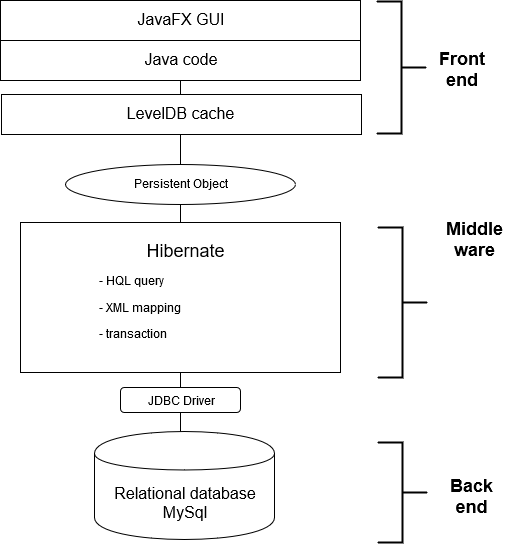
\includegraphics[height = 100mm]{./images/diagrams/architectureLevelDB.png} 
\vspace{6mm}
\captionof{figure}{Software architecture diagram\\}
\label{fig:architecture_diagram_levelDB}
\vspace{6mm}
\end{center}
\end{minipage}
LevelDB is a tool used to create a key-value database. It stores data under the form of key-value pairs locally in .sst file. Thanks to the property of those kind of databases we can think to set up a cache memory for our application using LevelDB.\\
We need to store information about professors/courses, with their relative comments, belonging to the same degree of the student that is actually logged. The idea is that the student will check those information more frequently than in the case of professors or courses of different degree.\\
When a student logs in, we retrieve and store the sequent data: professors (with their relative comments) and courses (with relative comments) of the same degree of the student. Those informations are then used to populate the tables needed during the normal operations of the application. We create the key for that data in the following way:
\begin{itemize}
\item For the professors’ data:\\ \textbf{professors:\$professor\_id:\$attribute\_name}\\ where the attributes are: name, surname and info.
\item For the subjects’ data:\\ \textbf{subjects:\$subject\_id:\$attribute\_name}\\ where the attributes are: name, credits and info.
\item For the professor’s comments data:\\ \textbf{prof\_comments:\$prof\_comments\_id:\$user\_id:\$professor\_id:\$attribute\_name}\\ where the attributes are: text and date.
\item For the subject’s comments data:\\ \textbf{subject\_comments:\$subject\_comment\_id:\$user\_id:\$subject\_id:\$attribute\_name}\\ where the attributes are: text and date.
\end{itemize}
\vspace{2mm}
Every time a users choose to see the informations about professors or subjects belonging to his same degree, we display the data stored locally. Once the user select a professor or a subject, the comment for that professor or for that subject are retrieved from the local file. \\
During the normal operation of the application, a student can add a new comment or update or modify one of his previously submitted comments.\\
When a user add a comment on one of the target objects (professors or subjects of his same degree), the new comment is first added onthe local file then the adding is propagated on the database. When a user modify or delete a comment, the action is only operated on the local file, when the user logs out those operations are then propagated on the relational database.\\
The admin, which is a super-user whith higher privileges, has to skip those step; in fact, the admin’s operations skip the local file and affect first the relational database, and then the key-value file, without the asynchronous steps.\\



\clearpage
% ----- MANUAL -----
\section{User Manual}
When you first run the application, the interface you get is the one in figure~\ref{fig:screen0}. 

\begin{figure}[h]
\centering
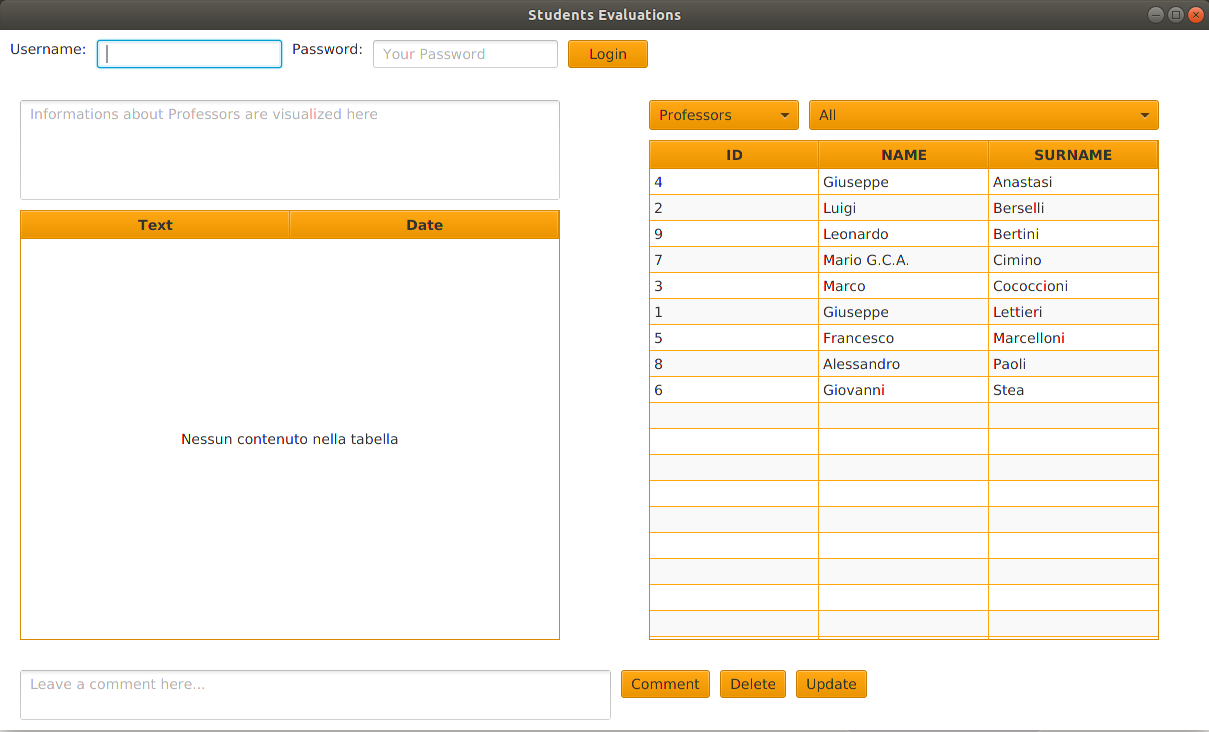
\includegraphics[width=0.88\textwidth]{images/screens/screen0}
\captionof{figure}{First view of the application}
\label{fig:screen0}
\end{figure}

The default display includes the list of all registered professors in the table on the right. You can choose to display the professors of a single degree course, using the drop-down menu on the right (fig.~\ref{fig:screen1}), or decide to view the list of subjects (fig.~\ref{fig:screen2}), for which is also available the degree course's filter. 

\begin{figure}[h]
\centering
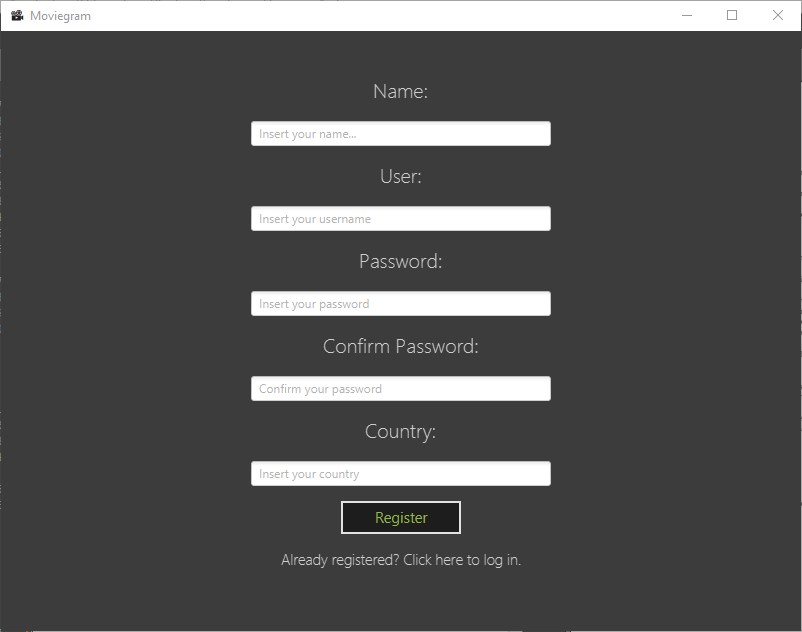
\includegraphics[width=0.88\textwidth]{images/screens/screen1}
\captionof{figure}{Selection of professors filtered by "Ingegneria Informatica" degree course}
\label{fig:screen1}
\end{figure}
\clearpage
\begin{figure}[h]
\centering
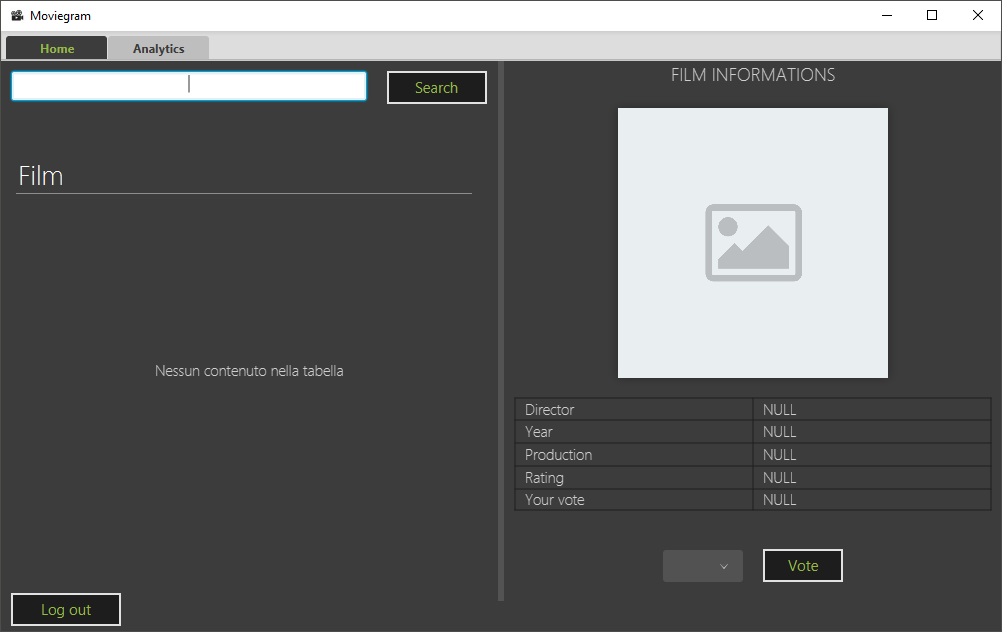
\includegraphics[width=0.88\textwidth]{images/screens/screen2}
\captionof{figure}{Selection of subjects}
\label{fig:screen2}
\end{figure}

If you have a registered account, you can log in to the application, so that the comments' operations aren't blocked. Enter your username and your password in the suited fields at the top and click on "Login" (fig.~\ref{fig:screenLogin}).
\begin{figure}[h]
\centering
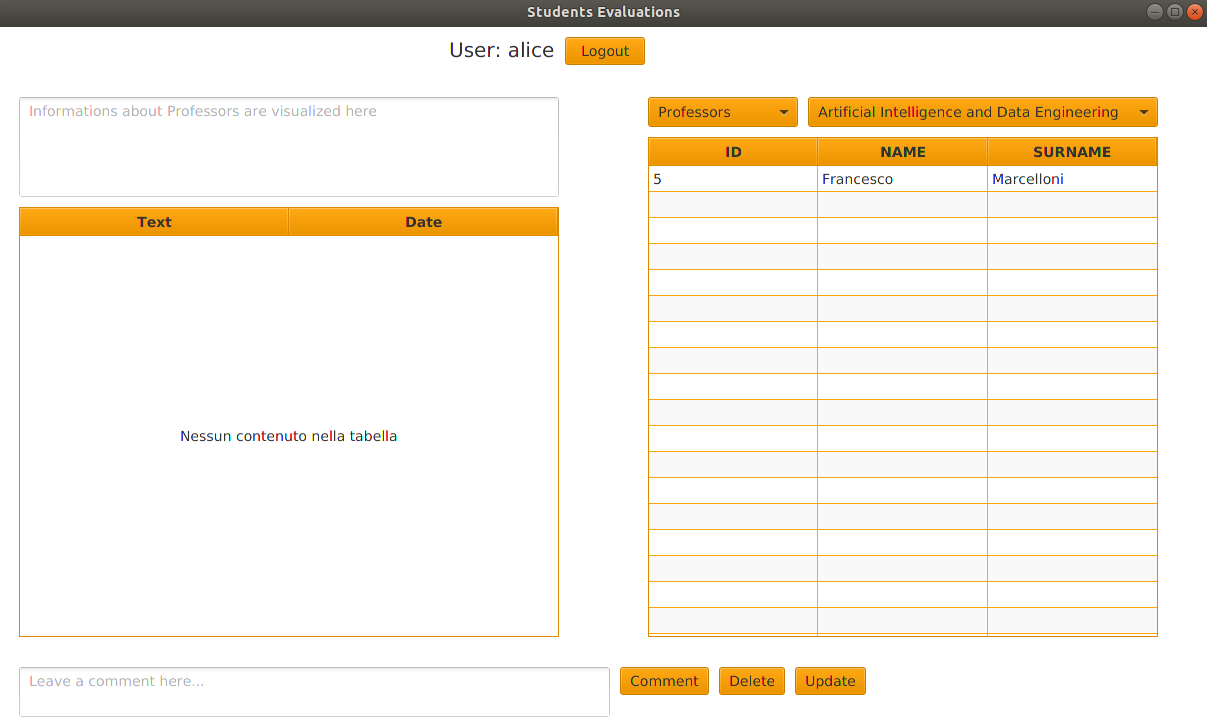
\includegraphics[width=0.88\textwidth]{images/screens/screenLogin}
\captionof{figure}{Application interface after the user "Alice" has logged in}
\label{fig:screenLogin}
\end{figure}

If you now want to be able to see the comments associated with a particular professor, you have to click on the name of the professor: in the table on the left the list of comments already received will appear (fig.~\ref{fig:screen3}). With this operation, you'll be able to visualize also the information related to that professor.

To leave a comment, you need to enter the text in the field below the table and then click on the "Comment" button. The result obtained from these operations is shown in fig.~\ref{fig:screen4}.

\begin{figure}
\centering
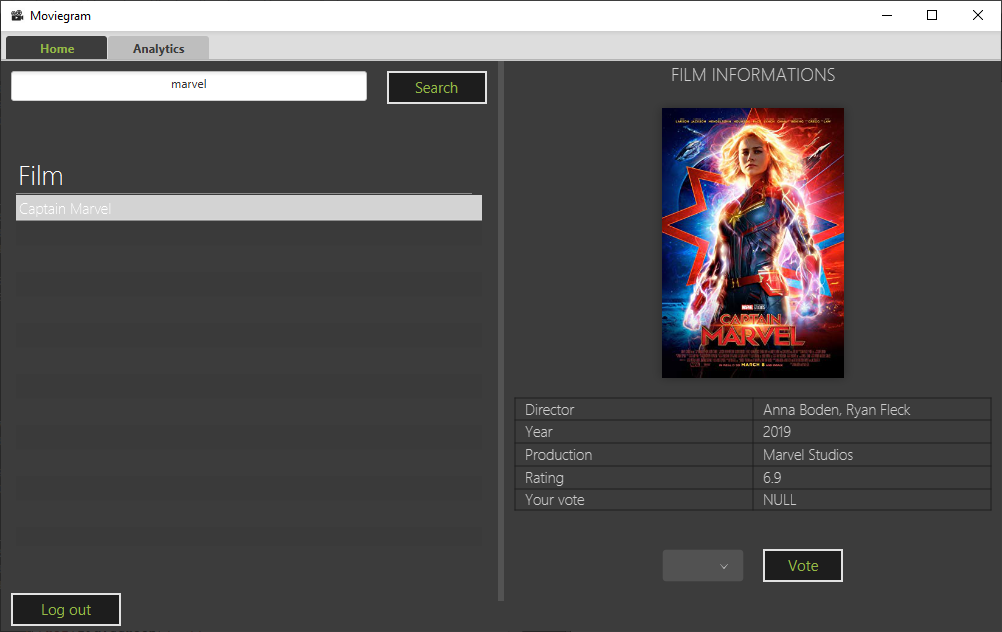
\includegraphics[width=0.9\textwidth]{images/screens/screen3}
\captionof{figure}{Displaying the comments related to a professor}
\label{fig:screen3}
\end{figure}

\begin{figure}
\centering
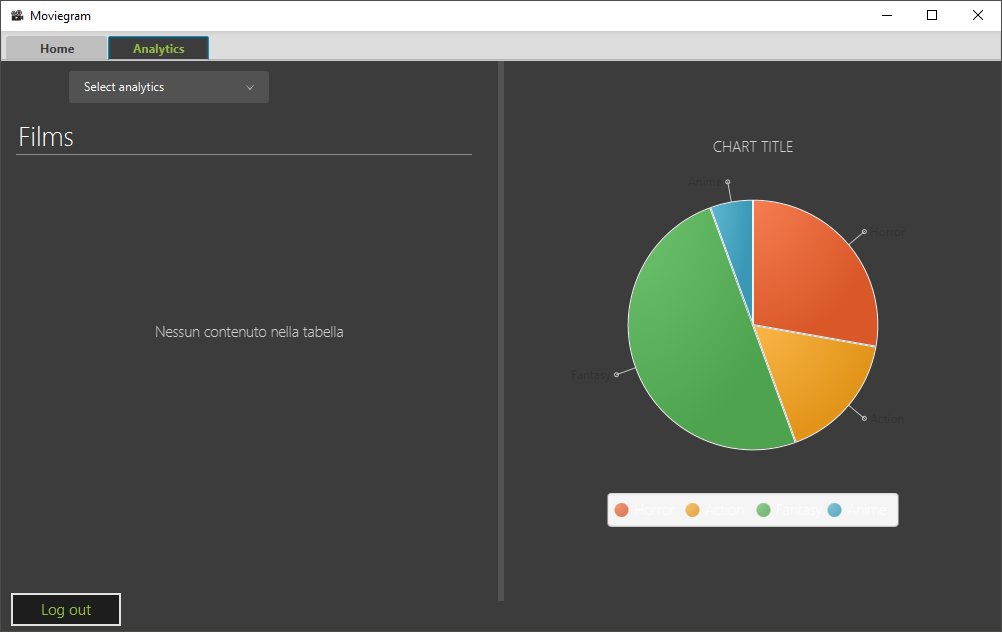
\includegraphics[width=0.9\textwidth]{images/screens/screen4}
\captionof{figure}{Interface after adding a comment}
\label{fig:screen4}
\end{figure}

You can also decide to modify the comment you just uploaded or another comment you made on a previous session. To do so, you need to click on the comment you want to update, change the text in the field below the table and then click on the "Update" button (fig.~\ref{fig:screen5}).
Finally you have the chance to delete your comment, by clicking on "Delete" after selecting it. Notice that you can modify or delete just the comments that you made.

The operations of adding, updating and deleting work as well for the the subjects' comments.
\begin{figure}[h]
\centering
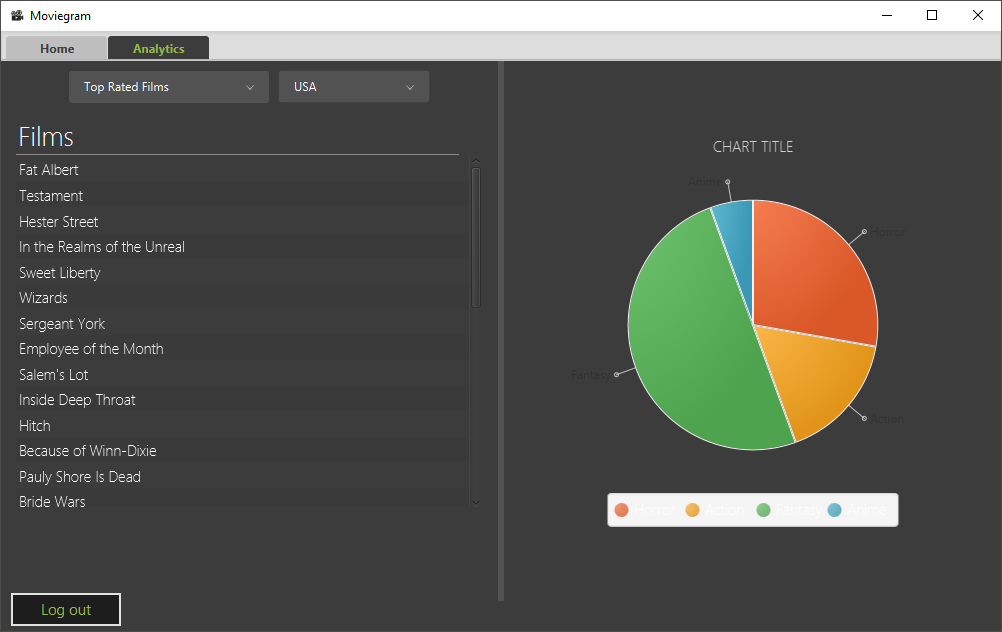
\includegraphics[width=0.88\textwidth]{images/screens/screen5}
\captionof{figure}{Interface after updating a comment}
\label{fig:screen5}
\end{figure}

To log out, just click on the appropriate button at the top, next to the user label.

Moreover, if you don't have a registered username, you can still browse through the application, search for professors 'and subjects' information and read all comments. You are just unable to leave or change any comments.

\clearpage
%ADIMN MANUAL%
\subsection{Admin Manual}
If you have an admin user, you are entitled to make changes both on the professors' and the subjects' lists. You need to log in inserting your username and password, and the application will recognize you as the administrator and show up the buttons for modifying the data (fig.~\ref{fig:adminLogin}).

\begin{figure}[h]
\centering
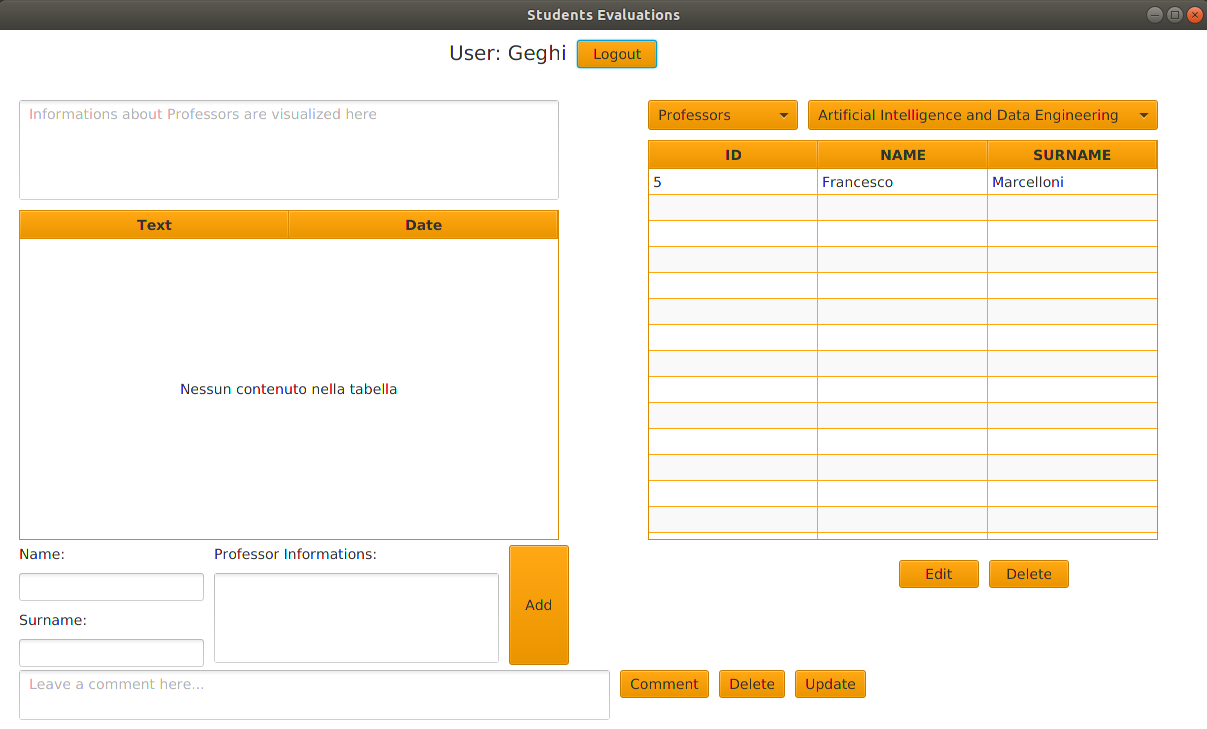
\includegraphics[width=0.88\textwidth]{images/screens/adminLogin}
\captionof{figure}{Interface after the administrator has logged in}
\label{fig:adminLogin}
\end{figure}

You can choose to add a new professor, using the input fields at the bottom left. You have to specify the name, surname, and description, then press the "Add" button (fig.~\ref{fig:admin1}).
\begin{figure}[h]
\centering
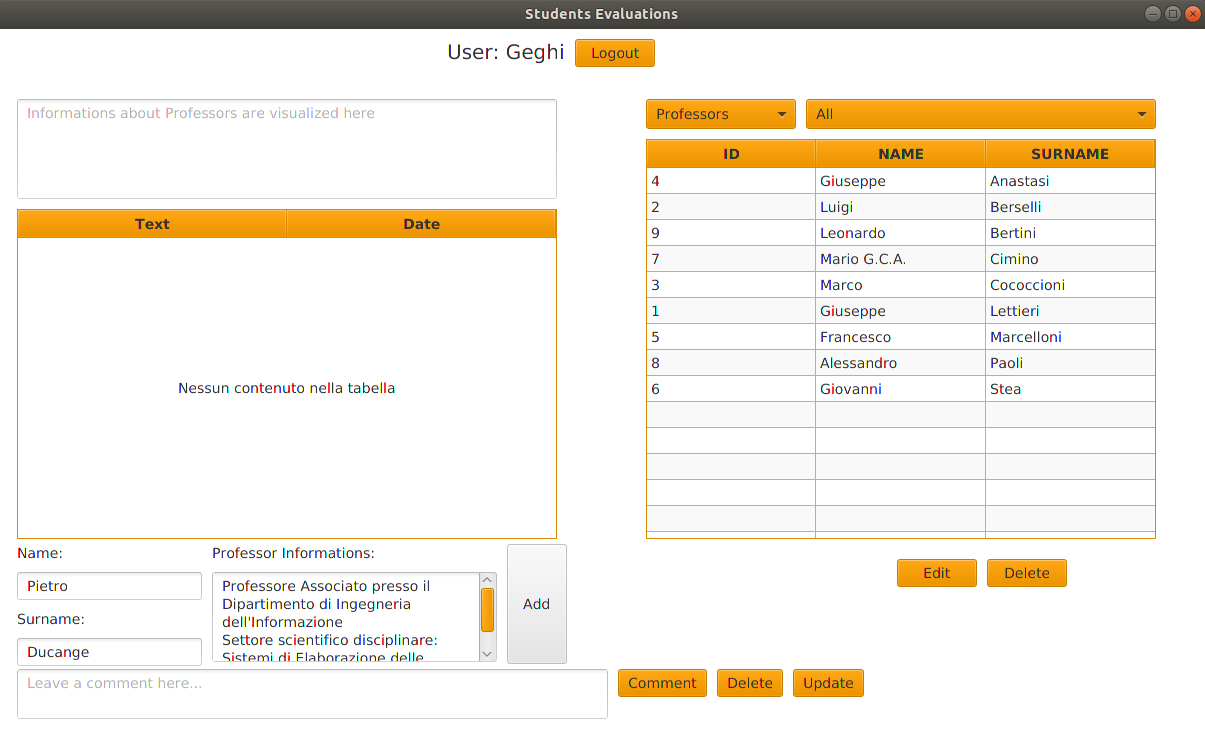
\includegraphics[width=0.88\textwidth]{images/screens/admin1}
\captionof{figure}{Adding a new professor}
\label{fig:admin1}
\end{figure}
\clearpage
You can also modify the data related to a professor: click on the professor you are interested in and change the information shown in the apposite input fields. Finally, you have the chance to delete a professor by clicking on the "Delete" button after selecting the wanted professor (fig.~\ref{fig:admin2}).
\begin{figure}[h]
\centering
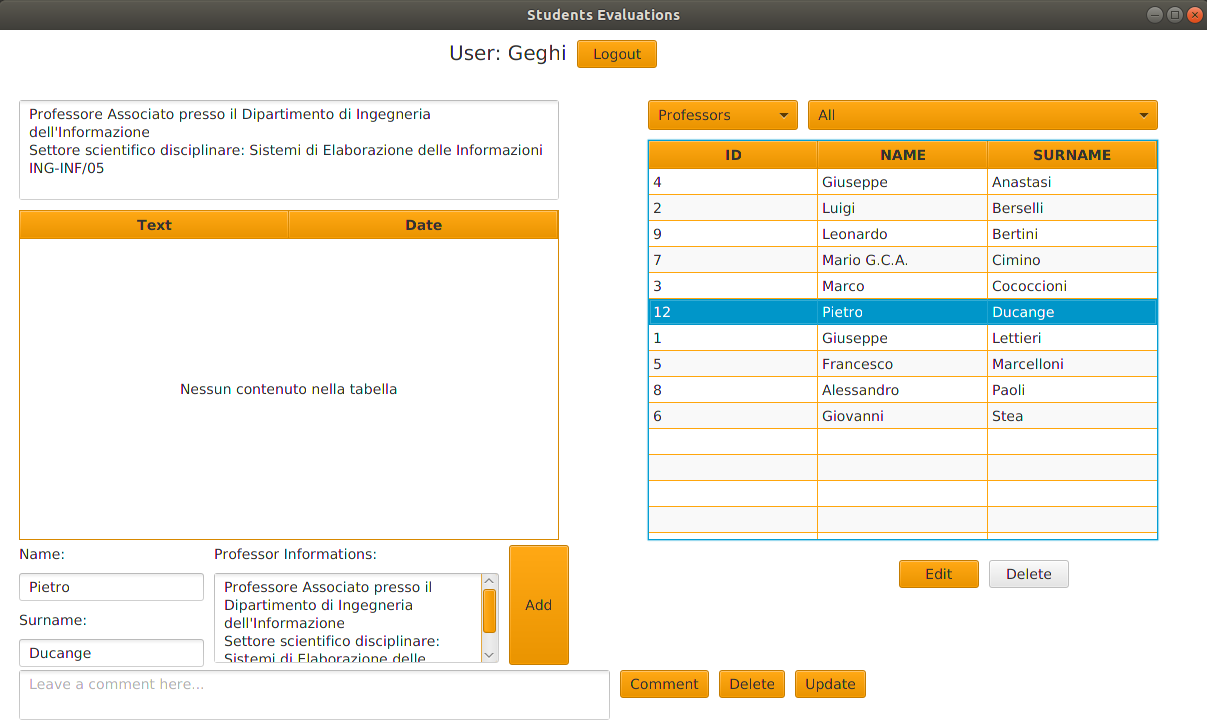
\includegraphics[width=0.88\textwidth]{images/screens/admin2}
\captionof{figure}{Screen of the application's interface from which you can either update or delete a professor}
\label{fig:admin2}
\end{figure}

All these operations are available for the subjects as well. The only difference is that when you want to add a new subject you also need to specify the id of the professor teaching it (or a list of ids, separeted by commas, if there are more professors teaching it). Moreover, you must have precisely displayed in the table the subjects of the same degree course of the new one (fig.~\ref{fig:admin3}).
\begin{figure}[h]
\centering
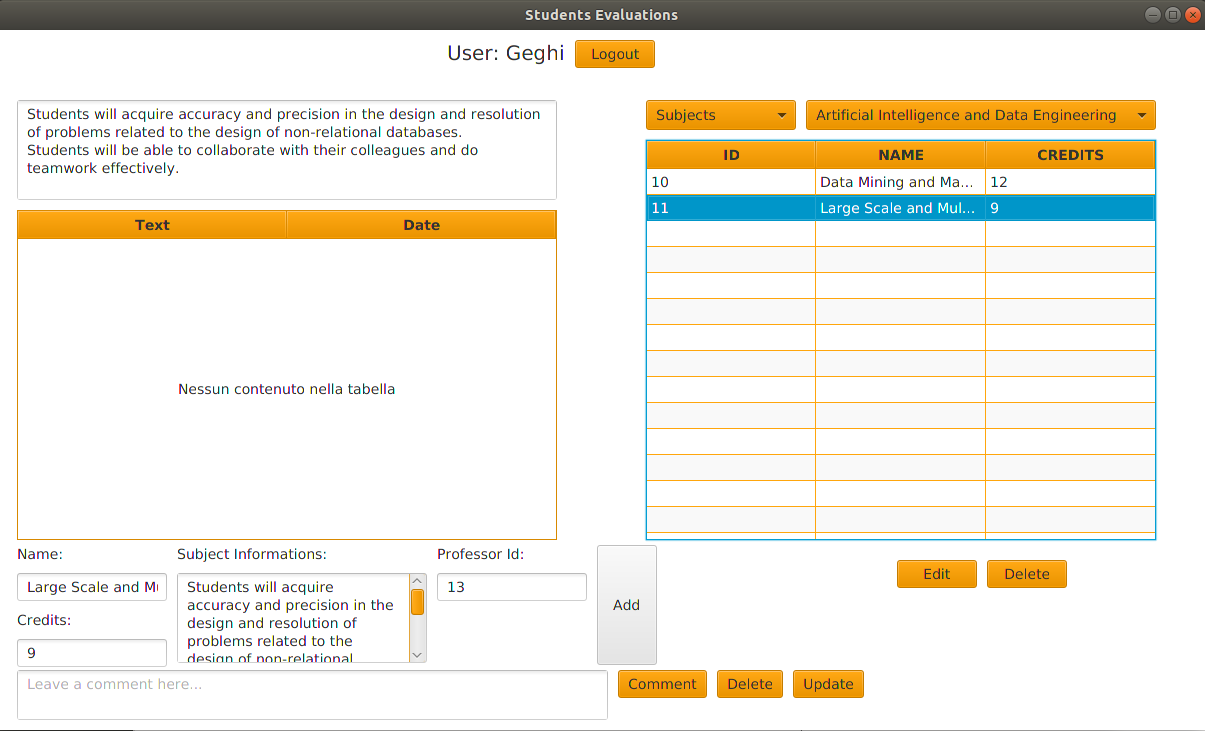
\includegraphics[width=0.88\textwidth]{images/screens/admin3}
\captionof{figure}{Interface after adding a new subject, ready to modify or delete it}
\label{fig:admin3}
\end{figure}
\clearpage
The administrator can delete comments posted by all the users, too. Just click on the comment and then on the "Delete" button (fig.~\ref{fig:admin4}).
\begin{figure}[h]
\centering
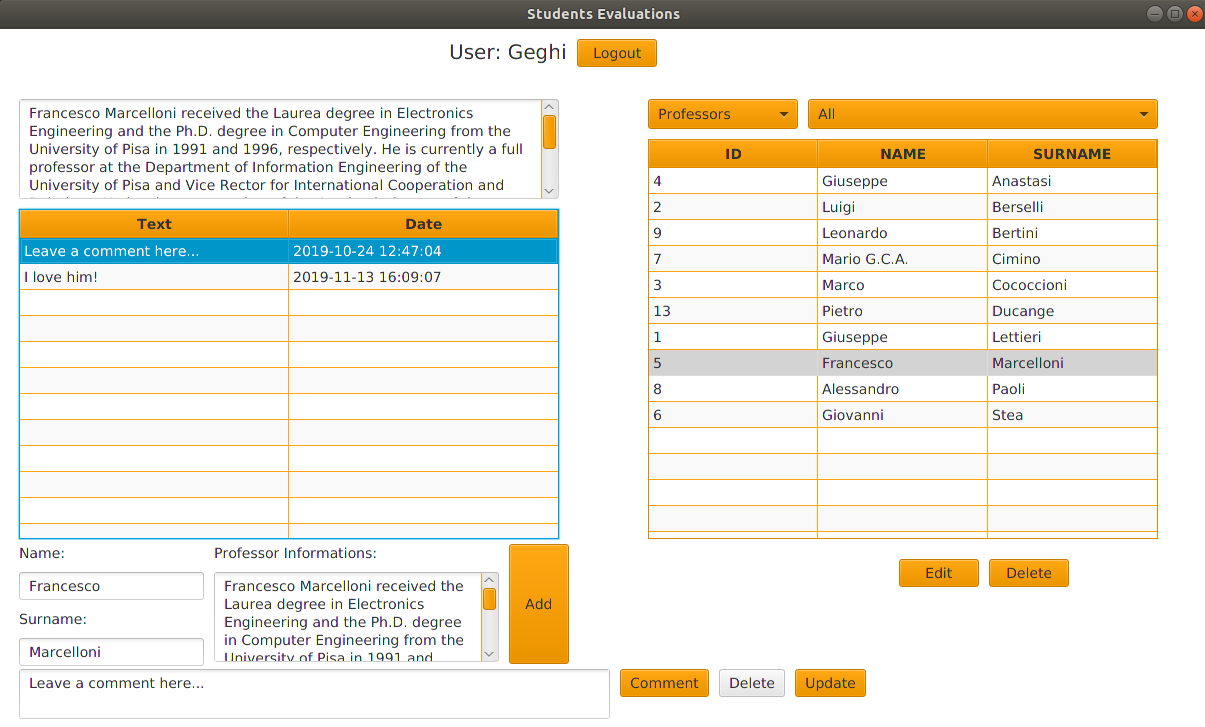
\includegraphics[width=0.88\textwidth]{images/screens/admin4}
\captionof{figure}{Screen of the application's interface from which the admin can delete a comment}
\label{fig:admin4}
\end{figure}

\fi

\end{document}






